\documentclass[xcolor=table]{beamer}

\usetheme[secheader,compress]{Madrid} %Primary theme

\usepackage{verbatim}
\usepackage{graphicx}

\graphicspath{{figures/}}

%% UTM Colors
\definecolor{UTMblue}{rgb}{0.043137, 0.137254, 0.254901}
\definecolor{UTMorange}{rgb}{1.0, 0.509803, 0}

\setbeamercolor{palette primary}{bg=UTMblue,fg=white}
\setbeamercolor{palette secondary}{bg=UTMblue,fg=white}
\setbeamercolor{palette tertiary}{bg=UTMblue,fg=white}
\setbeamercolor{palette quaternary}{bg=UTMblue,fg=white}
\setbeamercolor{structure}{fg=UTMblue} % itemize, enumerate, etc
\setbeamercolor{section in toc}{fg=UTMblue} % TOC sections
\setbeamercolor{title}{fg=UTMorange}

\setbeamercolor{subsection in head/foot}{bg=UTMorange,fg=white}

%%%%%%%%%%% BEGIN MACROS %%%%%%%%%%%%%%%%%%
% frameT: Frame with title
\newcommand{\frameT}[2]{\frame{\frametitle{#1} #2}}

% frameF: Fragile frame with title
\newcommand{\frameF}[2]{
  \begin{frame}[fragile]
    \frametitle{#1}
    #2
  \end{frame}
}

% frameTop: Frame aligned t the top
\newcommand{\frameTop}[2]{\frame[t]{\frametitle{#1} #2}}


\newcommand{\tab}{\hspace{1cm}}

\newcommand{\spaceor}{\hspace{5pt} \textbf{or} \hspace{5pt}}

%%%%%%%%%%% END MACROS %%%%%%%%%%%%%%%%%%%%



\begin{document}

\title{Kronos}

\author{Enrique Tejeda and Reily Stanford}
\institute{UT-Martin}
\date{\today}

%%%%%%%%%%% BEGIN TITLE %%%%%%%%%%%%%%%%%%
\frame{\titlepage}

 %\section{Outline}
%%%%%%%%%%%% END TITLE  %%%%%%%%%%%%%%%%%%


\section{Introduction}

\frameT{Motivation} {
  \begin{itemize}
    \item Paranautical Activity - A roguelike FPS with a low-poly art style
    \medskip
	\begin{center}
		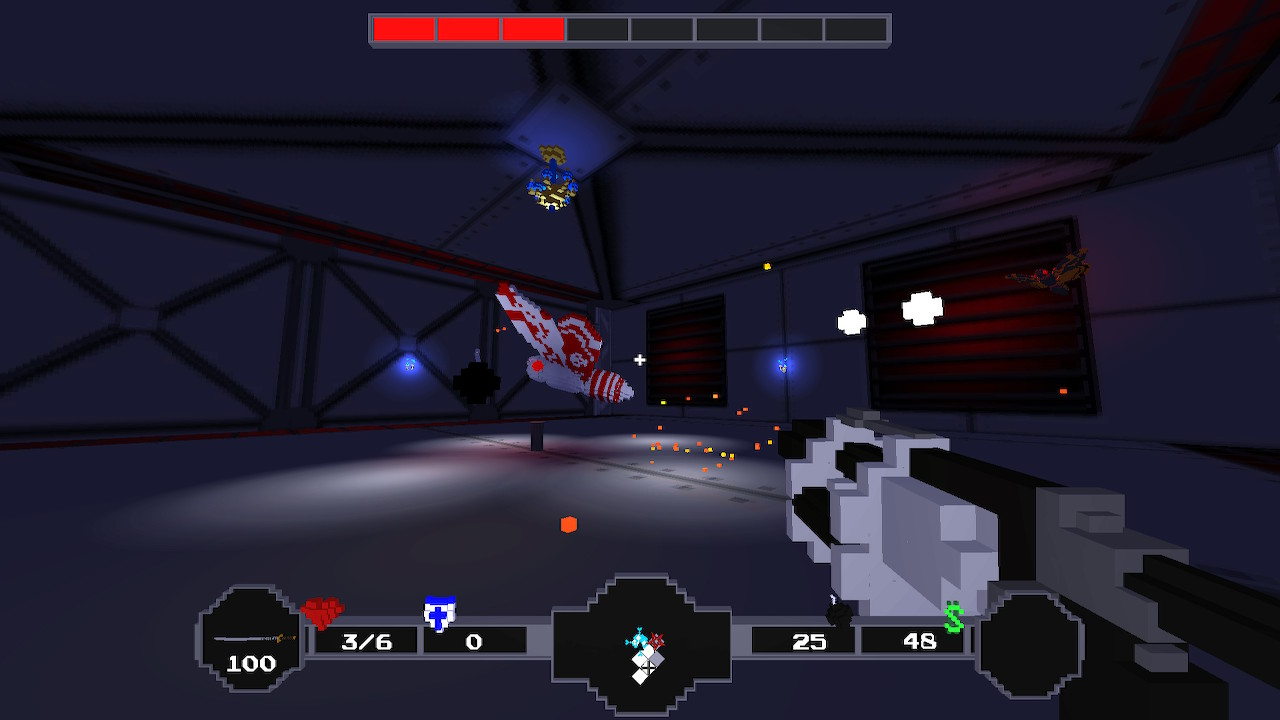
\includegraphics[scale=0.15]{paranautical_activity}
	\end{center}	    
      \smallskip
    \item Experimentation with VR technologies
      \medskip
    \item Learning game design elements with Unreal Engine
  \end{itemize}
}

\frameT{Story} {
	\begin{itemize}
		\item Someone has broken the rules of time
		\bigskip
		\item Timeline is scrambled, up to Kronos to repair it
		\bigskip
		\item Kronos manipulates time to assist in restoring time
	\end{itemize}
}

\frameT{Technology} {
	\begin{itemize}
		\item Created using Unreal Engine 5
		\bigskip
		\item Programmed using Unreal's Blueprints
		\medskip
		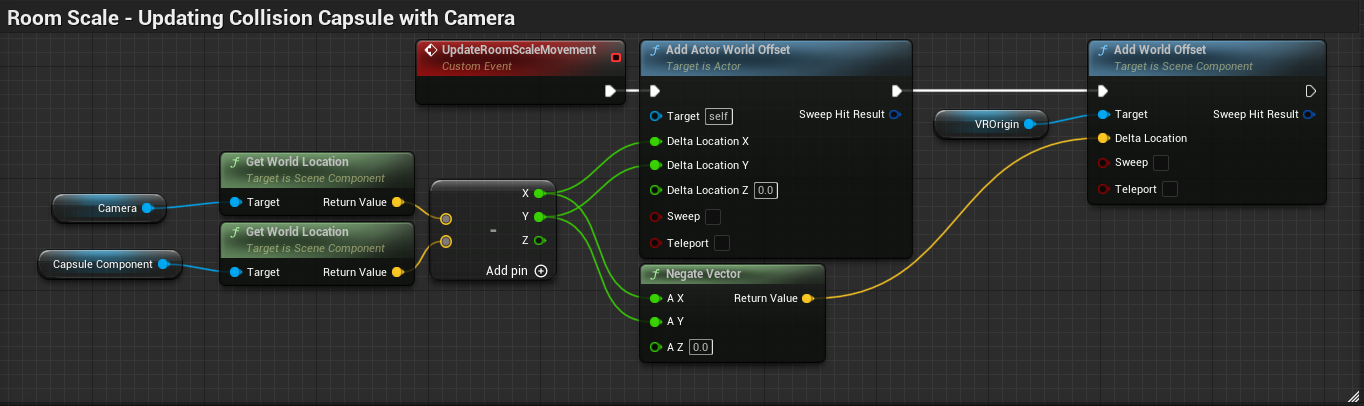
\includegraphics[scale=0.22]{blueprint}
		\smallskip
		\item Programmed with C++ for complex features
	\end{itemize}
}

\section{Details}

\frameT{Gameplay} {
	\begin{itemize}
		\item Kronos is a VR FPS roguelike
		\bigskip
		\item Each level is a different time period
		\bigskip
		\item Enemies and bosses will reflect the era of the level
		\bigskip
		\item Kronos is able to bring weapons across levels
	\end{itemize}
}

\frameT{Demonstration} {
	\begin{center}
		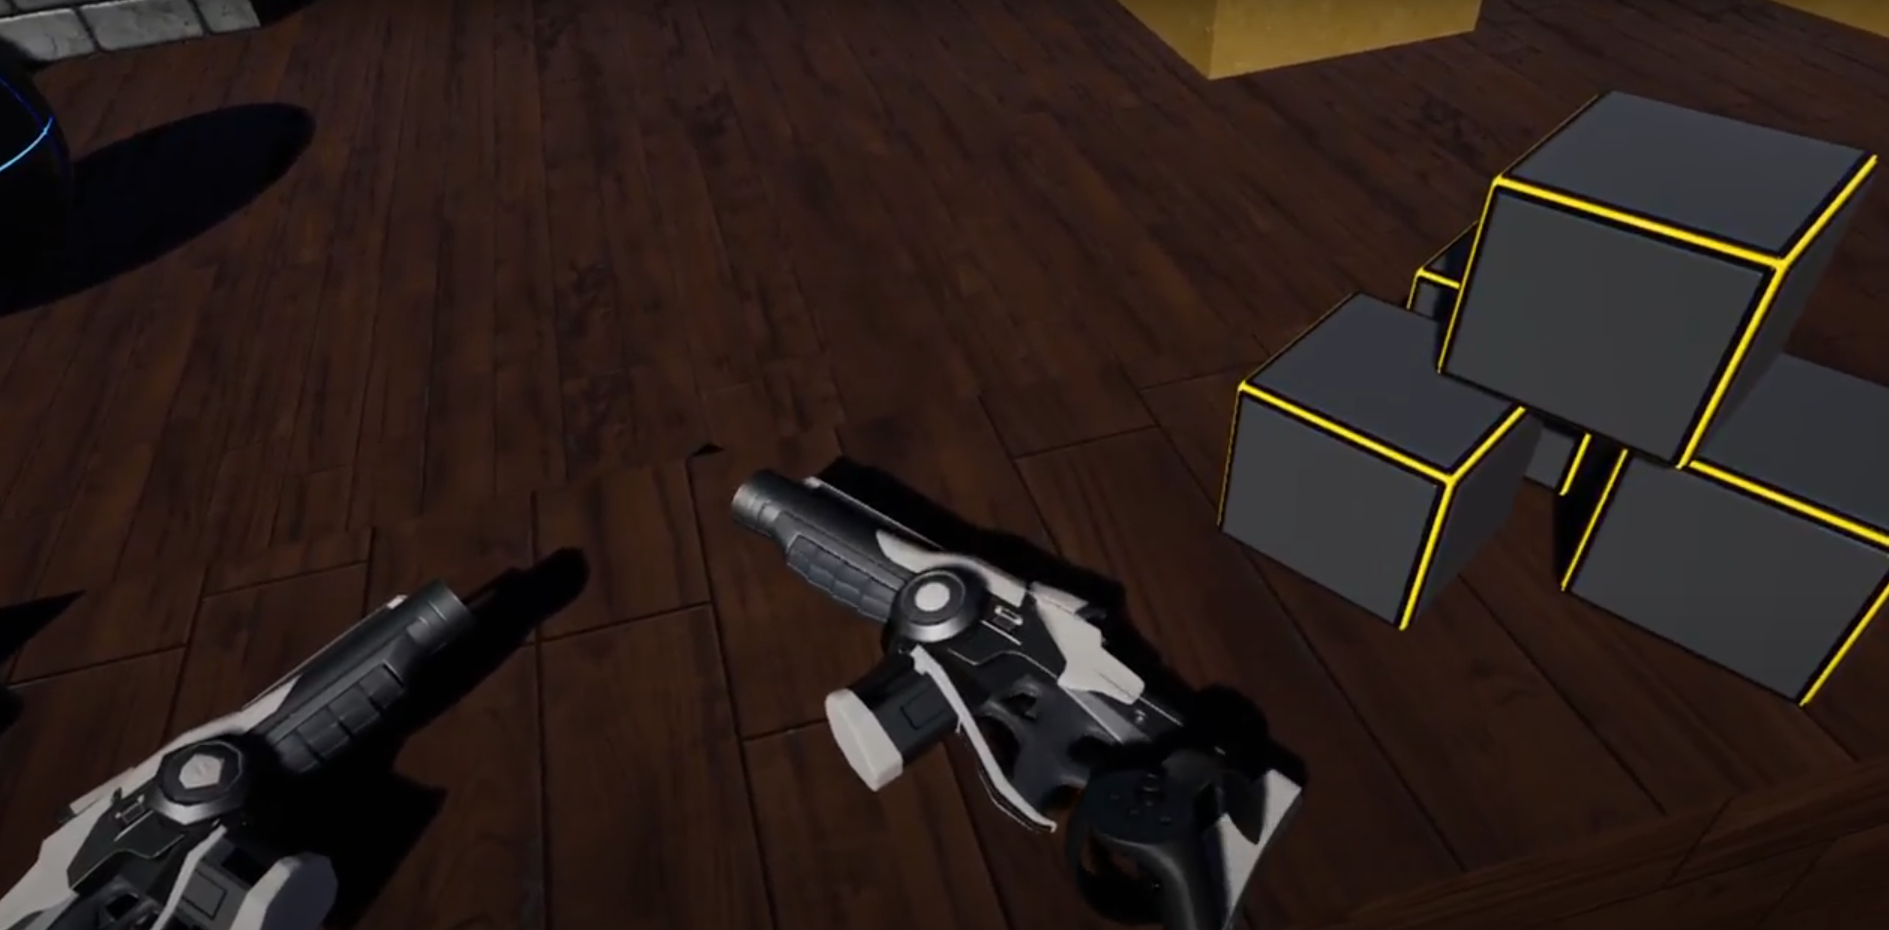
\includegraphics[scale=0.3]{demo}
	\end{center}
}

\frameT{Trials and Tribulations} {
	\begin{figure}[ht]
    	\begin{minipage}[b]{0.3\linewidth}
      		\centering
      		\begin{itemize}
      			\item Movement
				\bigskip
				\item Sprite Management
				\bigskip
				\item Dungeon Creating Plugin
      		\end{itemize}
    	\end{minipage}
    	\hspace{0.5cm}
    	\begin{minipage}[b]{0.5\linewidth}
    	\centering
    			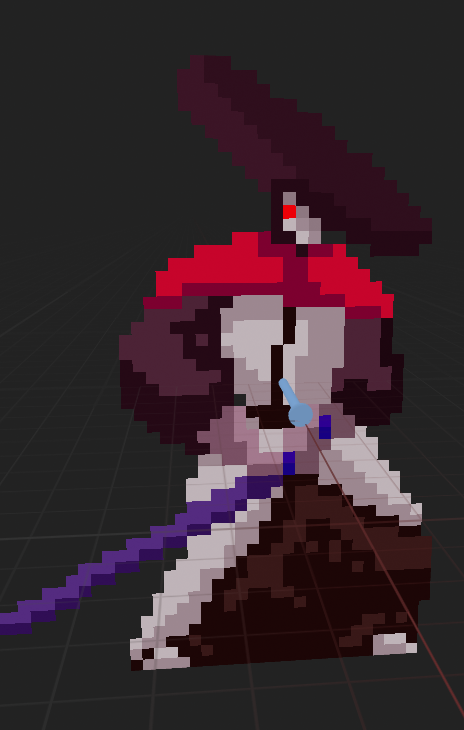
\includegraphics[scale=0.16]{sprite.png}
    	\end{minipage}
  	\end{figure}
}

\section{Conclusion}

\frameT{Future Work} {
	\begin{itemize}
		\item Creating more room layouts and floors
		\bigskip
		\item Adding verticality
		\bigskip
		\item More enemies and bosses
		\bigskip
		\item Items
	\end{itemize}
}

\frameT{Feedback} {
	\begin{itemize}
		\item Any questions?
		\bigskip
		\item Project repo: https://github.com/enrgteje/Kronos
	\end{itemize}
	\bigskip
	\bigskip
	\centering
	Contact us:
		\begin{figure}[ht]
    		\begin{minipage}[b]{0.4\linewidth}
      			\centering
      			enrgteje@ut.utm.edu
      			github.com/enrgteje
    		\end{minipage}
    		\hspace{0.5cm}
    		\begin{minipage}[b]{0.4\linewidth}
      			\centering
      			rstanfo1@ut.utm.edu
      			github.com/reilys
    		\end{minipage}
  		\end{figure}
	
}


%\frameT{Project Goals} {
%  Described what you are trying to accomplish, including ``stretch'' goals.
%}

%\section{Sections--a useful organizational tool.}
%
%\frameT{}{
%}
%
%
%
%\begin{frame}[fragile]
%\frametitle{Family Tree Knowledge Base}
%Facts:
%\begin{verbatim}
%Verbatim is a great way of enumerating code/algorithmic ideas.
%\end{verbatim}
%\end{frame}
%
%
%\frameT{How to include images} {
%  %% \includegraphics[width=.7\linewidth]{figures/image.pdf}
%}
%
%
%\begin{frame}[fragile]
%  \frametitle{Social Network Graph}
%  \begin{figure}[ht]
%    \begin{minipage}[b]{0.53\linewidth}
%      \centering
%      Minipages are a great way to
%    \end{minipage}
%    \hspace{0.5cm}
%    \begin{minipage}[b]{0.4\linewidth}
%      \centering
%      Line up side-by-side content.
%
%    \end{minipage}
%  \end{figure}
%  
%\end{frame}
%
%
%\frameT{Results} {
%  Describe any results of your work here.
%
%  \bigskip
%
%  Things that worked?
%
%  \bigskip
%
%  Things that didn't work?
%}
%
%\frameT{Conclusions} {
%  Some bullet points here to wrap things up.
%}
%
%\frameT{Any Questions?} {
%  
%  \begin{center}
%    Questions?
%  \end{center}
%  \begin{center}
%    Comments?
%  \end{center}
%
%  \bigskip
%
%  Further project/author information:
%  \begin{center}
%    
\includegraphics[width=4cm]{6AnLddq.png}
%  \end{center}
%}

%\frameF{fragile test} {
%}

%% \frameF{Prolog Family Tree} {
%% \begin{verbatim}
%% hello
%% \end{verbatim}



%% }

%Empty Page
%\frameT{Frame 1}{
%}  


\end{document}
